%
%	Configure LaTeX to produce a PDF presentation using the beamer class
%

\documentclass[ignorenonframetext,11pt]{beamer}
\usepackage[ngerman]{babel}
\usepackage[utf8]{inputenc}		% For UTF-8 support
\usepackage[T1]{fontenc}

\usepackage{graphicx}


\usepackage{beamerthemesplit}
\usepackage{patchcmd}
\usepackage{tabulary}		% Support longer table cells
\usepackage{booktabs}		% Support better tables
\usepackage[sort&compress]{natbib}

\usepackage{framed}			% Allow background color for images
\definecolor{shadecolor}{named}{white}


\usepackage{subfigure}

\let\oldSubtitle\subtitle


% Configure default metadata
\input{mmd-default-metadata}


%\AtBeginSection[]
%{
 %\begin{frame}
    %\frametitle{Inhalt}
	%\tableofcontents %[currentsection,currentsubsection]
   %\end{frame}
%}


\long\def\citefoot#1{\let\thefootnote\relax\footnotetext{\citet{#1}} }

\def\mytitle{File Network: Reflexion der Usability Guidelines}
\def\myauthor{Anastasia Kazakova, Bengt Lüers}
\def\latexmode{beamer}
\def\latexxslt{beamer}
\def\theme{keynote-IntSysTheme}
\input{mmd-natbib-plain}
\def\bibliostyle{chicago}
%
%	Get ready for the actual document
%

%
% Use default MMD metadata for beamer equivalents
%

\ifx\subtitle\undefined
\else
	\oldSubtitle{\subtitle}
\fi

\ifx\affiliation\undefined
\else
	\institute{\affiliation}
\fi

\ifx\mydate\undefined
	\def\mydate{\today}
\else
	\date{\mydate}
\fi

\ifx\event\undefined
\else
	\date[\mydate]{\mydate~ / \event }
\fi


%\input{mmd-title}

% Show "current/total" slide counter in footer
\title[\mytitle\hspace{2em}\insertframenumber/
\inserttotalframenumber]{\mytitle}


\author{\myauthor}
\addtolength{\parskip}{\baselineskip}

\ifx\theme\undefined
\else
	\usetheme{\theme}
\fi

\begin{document}
\frame[plain]{\setlength\parskip{0pt}\titlepage}

\# \#

\section{Goldene Regeln}
\label{goldeneregeln}

\begin{frame}

\frametitle{Golden Rule 1: Consistency}
\label{goldenrule1:consistency}

\begin{itemize}
\item Dateien durch Symbole (Dateityp) und Name

\item Kreise zum Zusammenfassen

\item Verbindungen zw. den Dateien

\item Pie-Menues (?)

\end{itemize}

\end{frame}

\begin{frame}

\frametitle{Beispiel}
\label{beispiel}

\begin{figure}[htbp]
\centering
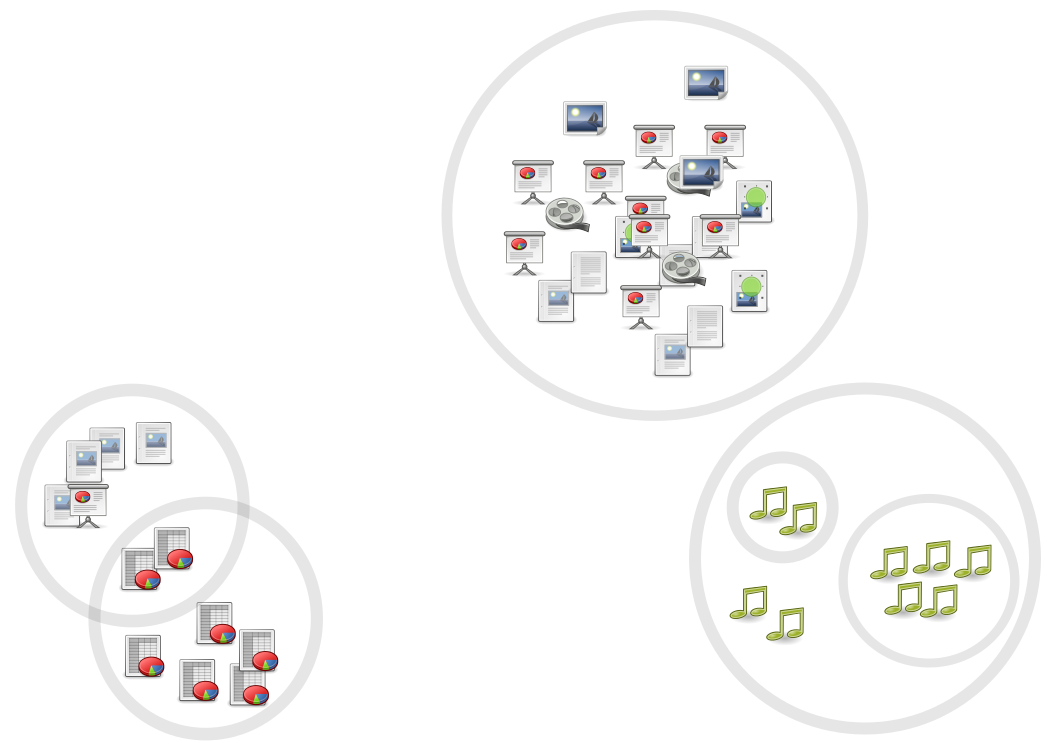
\includegraphics[keepaspectratio,width=\textwidth,height=0.75\textheight]{01.png}
\label{}
\end{figure}


\end{frame}

\begin{frame}

\frametitle{Golden Rule 3: Informative Feedback}
\label{goldenrule3:informativefeedback}

\begin{itemize}
\item Hervorheben von erstellten Verbindungen

\item Hervorheben von eingeordneten Kreisen

\item Permanentes Anzeigen der Dateien

\end{itemize}

\end{frame}

\begin{frame}

\frametitle{Beispiel}
\label{beispiel}

\begin{figure}[htbp]
\centering
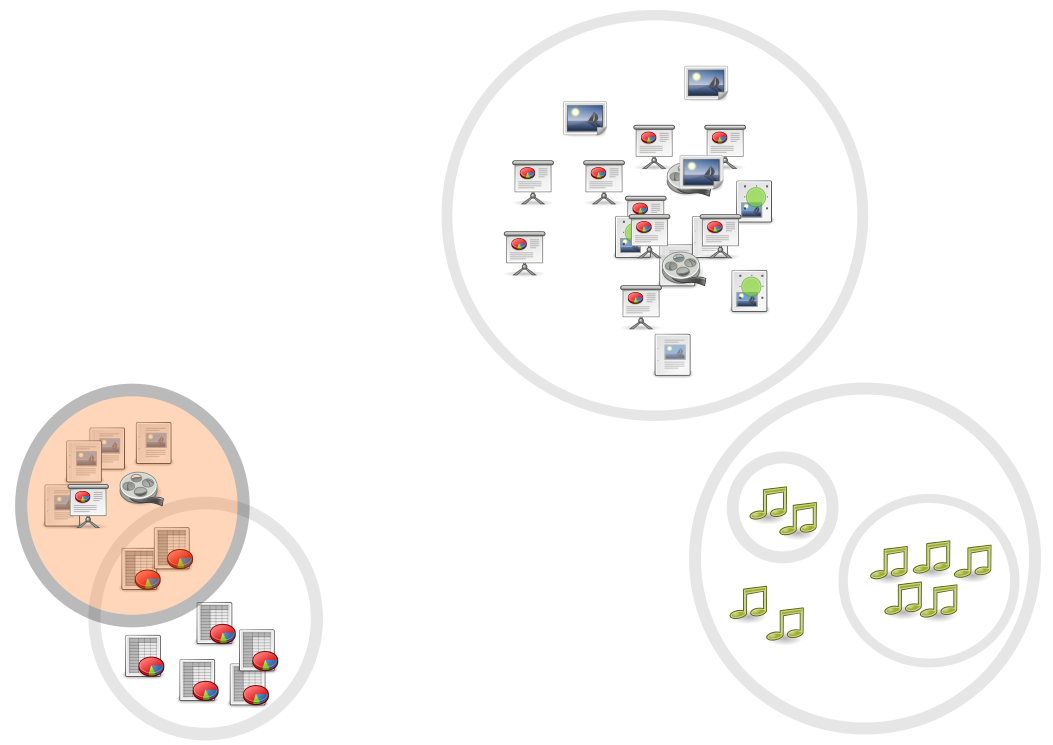
\includegraphics[keepaspectratio,width=\textwidth,height=0.75\textheight]{02.png}
\label{}
\end{figure}


\end{frame}

\begin{frame}

\frametitle{Golden Rule 5: Prevent Errors}
\label{goldenrule5:preventerrors}

\begin{itemize}
\item Durch das Feedback

\begin{itemize}
\item nachvollziehbare Aktionen

\end{itemize}

\item Snappen

\begin{itemize}
\item Halten in der ungefähren Richtung reicht

\end{itemize}

\end{itemize}

\end{frame}

\begin{frame}

\frametitle{Golden Rule 7: User Control}
\label{goldenrule7:usercontrol}

\begin{itemize}
\item in der Lern-\slash Anfangsphase, ansonsten

\item brechen wir,

\item denn:

\begin{itemize}
\item Maschinelles Lernen

\item Bereitschaft sich helfen zu lassen

\end{itemize}

\end{itemize}

\end{frame}

\section{Guidelines}
\label{guidelines}

\begin{frame}

\frametitle{Organizing the Display}
\label{organizingthedisplay}

\begin{itemize}
\item Aktuelle Dateien in der Mitte

\end{itemize}

\end{frame}

\begin{frame}

\frametitle{Beispiel}
\label{beispiel}

\begin{figure}[htbp]
\centering
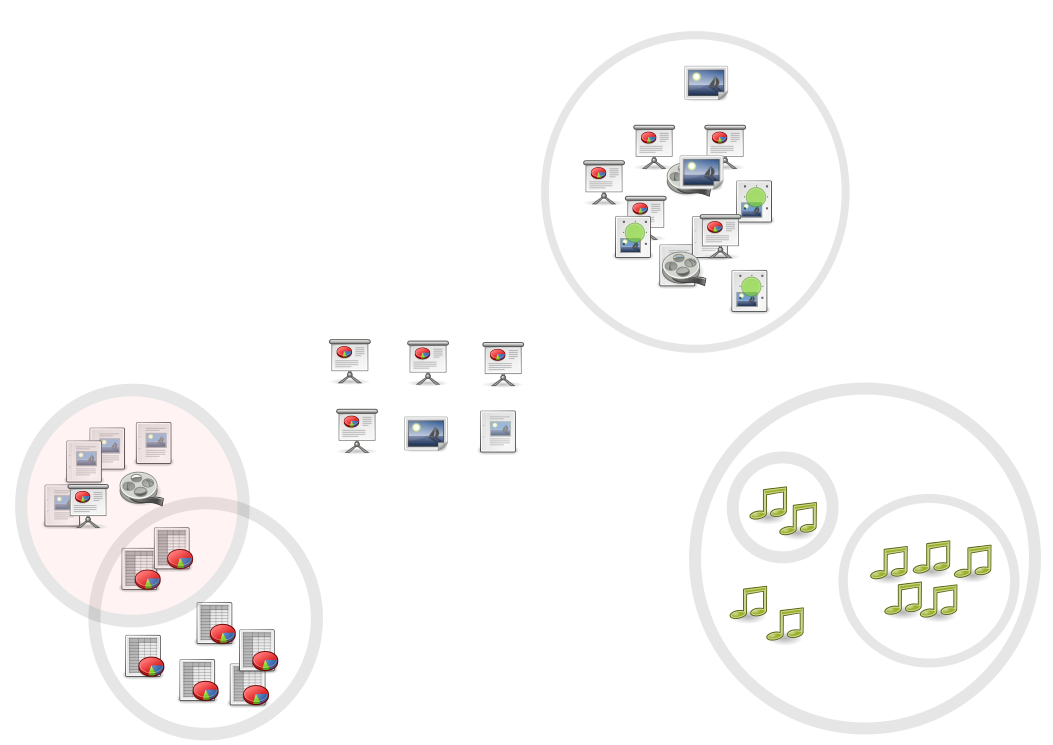
\includegraphics[keepaspectratio,width=\textwidth,height=0.75\textheight]{03.png}
\label{}
\end{figure}


\end{frame}

\begin{frame}

\frametitle{Getting the User's Attention}
\label{gettingtheusersattention}

\begin{itemize}
\item Verbindungen

\begin{itemize}
\item keine Intensität =$>$ nicht vorhanden

\item Intensität 1 =$>$ Vorhanden

\item Intensität 2 =$>$ Hervorgehoben

\end{itemize}

\item Dateien

\begin{itemize}
\item groß =$>$ aktuell

\item klein =$>$ veraltet

\end{itemize}

\item Kreise

\begin{itemize}
\item Farbe für Identifikation

\item Mischfarben für Überlappungen

\end{itemize}

\end{itemize}

\end{frame}

\begin{frame}

\frametitle{Beispiel}
\label{beispiel}

\begin{figure}[htbp]
\centering
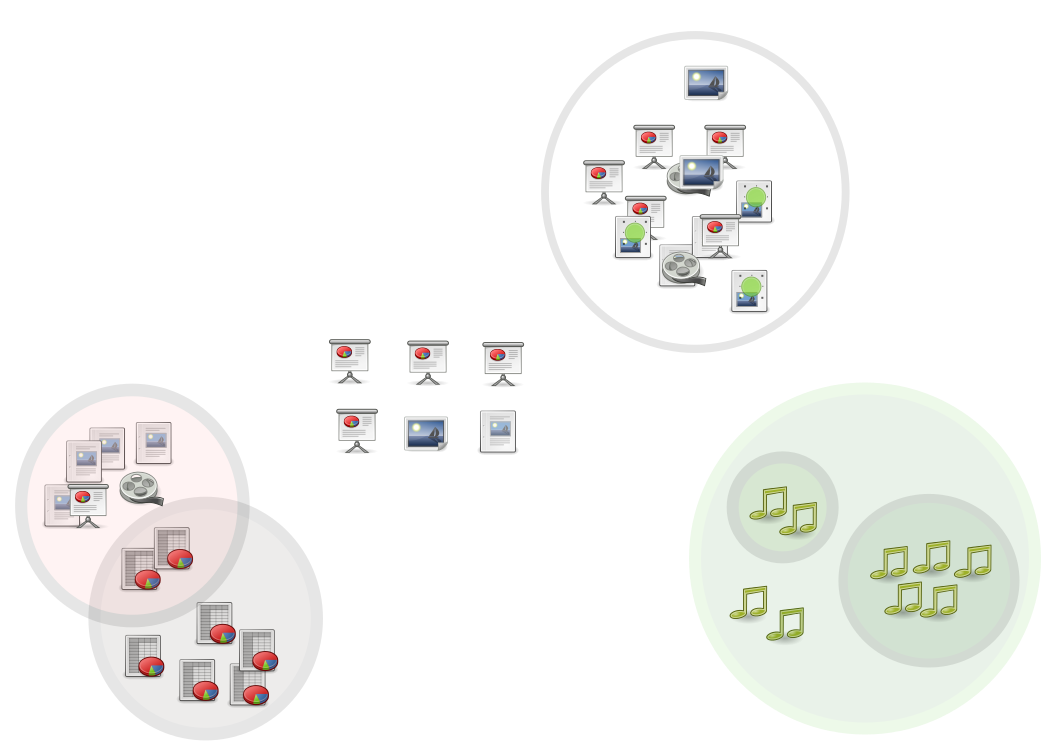
\includegraphics[keepaspectratio,width=\textwidth,height=0.75\textheight]{04.png}
\label{}
\end{figure}


\end{frame}

\begin{frame}

\frametitle{Beispiel}
\label{beispiel}

\begin{figure}[htbp]
\centering
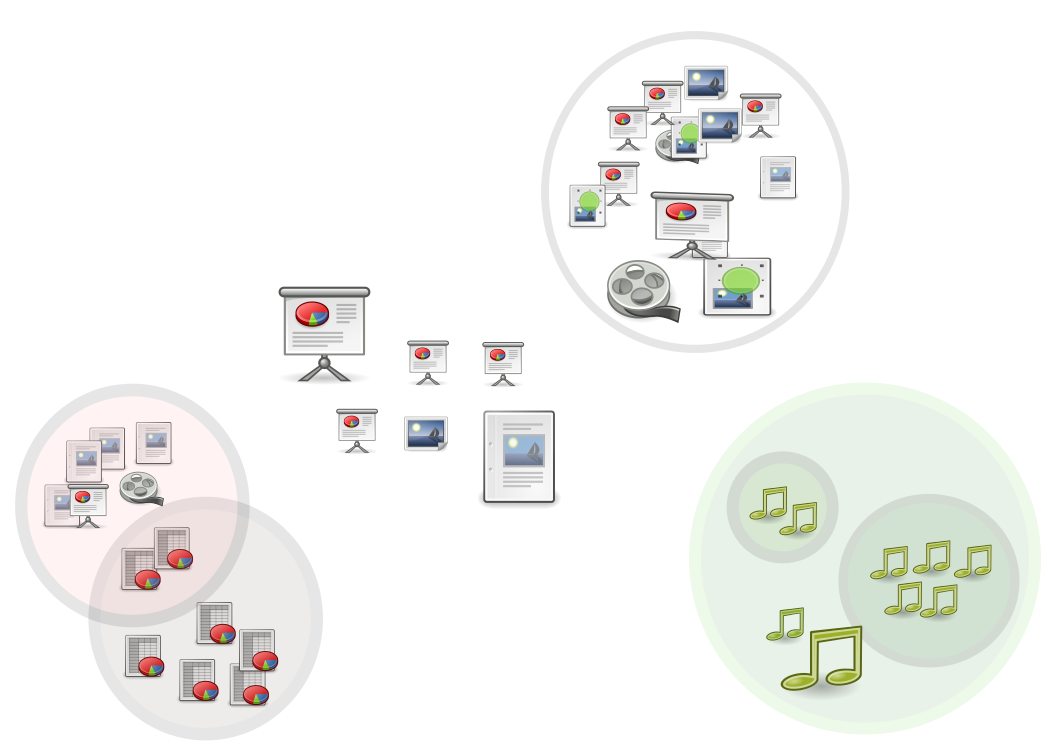
\includegraphics[keepaspectratio,width=\textwidth,height=0.75\textheight]{05.png}
\label{}
\end{figure}


\end{frame}

\section{Standards}
\label{standards}

\begin{frame}

\frametitle{Conformity with User's Expectations}
\label{conformitywithusersexpectations}

\begin{itemize}
\item Gezogene Datei landet ungefähr da, wo sie losgelassen wurde

\end{itemize}

\end{frame}

\begin{frame}

\frametitle{Beispiel}
\label{beispiel}

\begin{figure}[htbp]
\centering
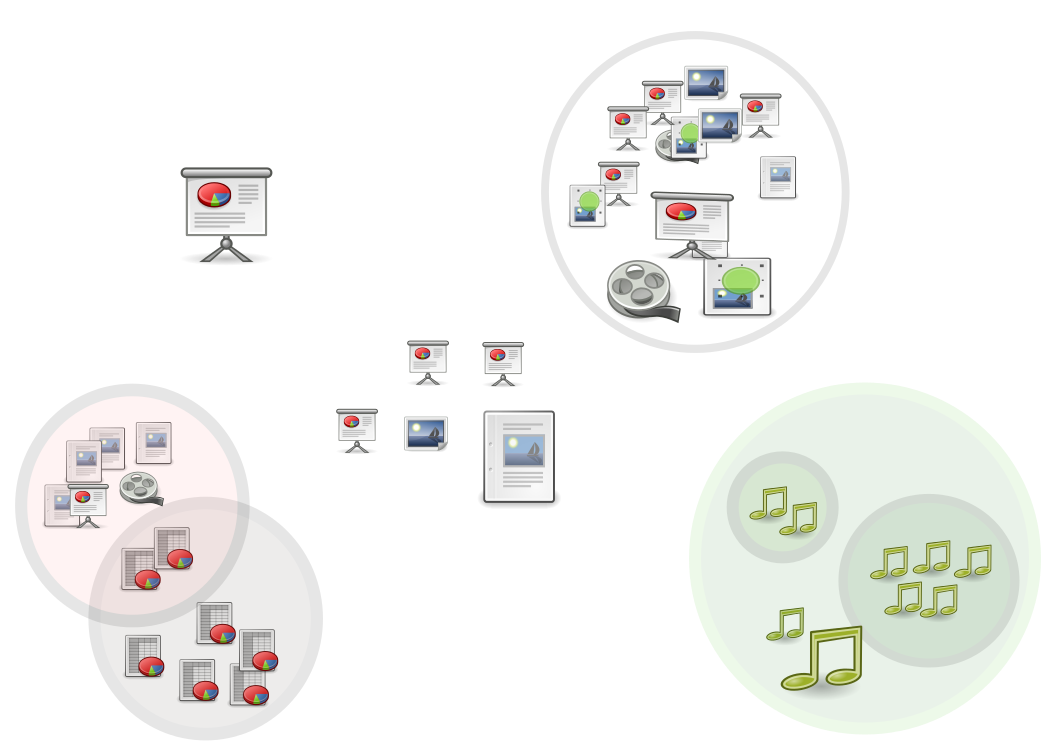
\includegraphics[keepaspectratio,width=\textwidth,height=0.75\textheight]{06.png}
\label{}
\end{figure}


\end{frame}

\begin{frame}

\frametitle{Beispiel}
\label{beispiel}

\begin{figure}[htbp]
\centering
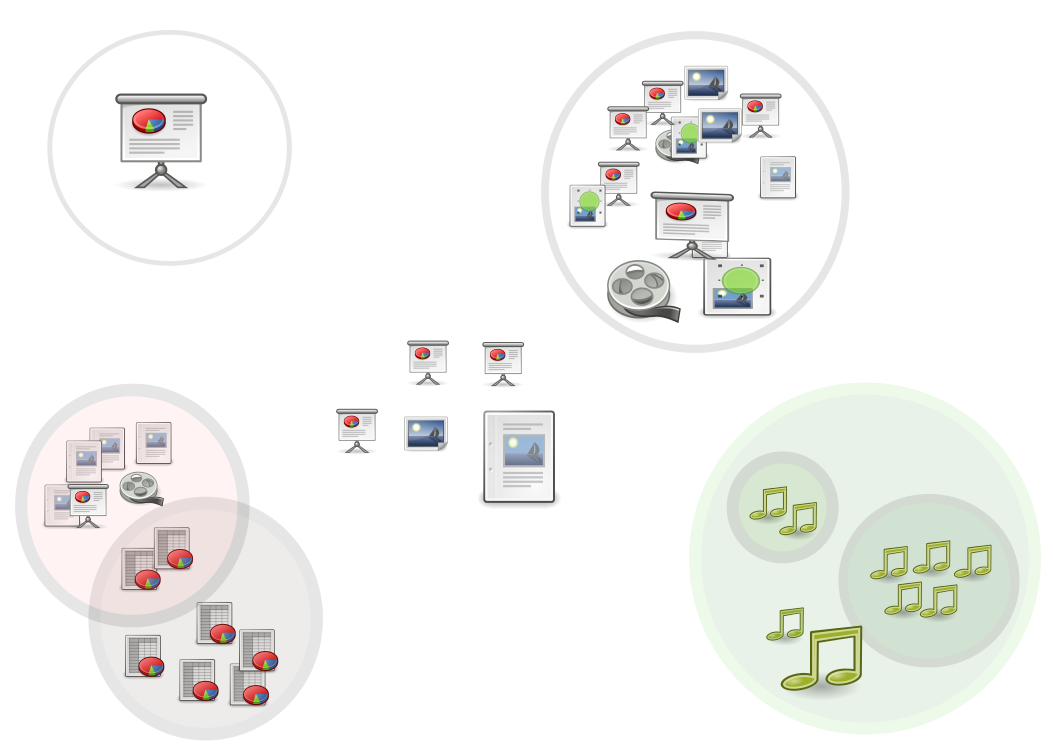
\includegraphics[keepaspectratio,width=\textwidth,height=0.75\textheight]{07.png}
\label{}
\end{figure}


\end{frame}

\begin{frame}

\frametitle{Error Tolerance}
\label{errortolerance}

\begin{itemize}
\item Snapping

\item Instant Feedback

\end{itemize}

\end{frame}

\begin{frame}

\frametitle{Suitability for Individualization}
\label{suitabilityforindividualization}

\begin{itemize}
\item Farbauswahl durch Nutzer

\end{itemize}

\end{frame}

\begin{frame}

\frametitle{Vielen Dank für die Aufmerksamkeit!}
\label{vielendankfrdieaufmerksamkeit}

\textbf{Fragen?}

\end{frame}

\mode<all>
%
%	MultiMarkdown beamer class footer file
%

% Back Matter
\if@mainmatter
\backmatter
\fi

\ifx\bibliocommand\undefined
\else
	\part{Literatur}
	\begin{frame}[allowframebreaks]
	\frametitle{Quellen}
	\bibliographystyle{\bibliostyle}
	\def\newblock{}
	\bibliocommand
	\end{frame}
\fi


\end{document}\mode*

